
\documentclass[12pt]{article}
\usepackage{amsmath,amssymb,bm}
\usepackage{geometry}
\geometry{margin=1in}
\usepackage{siunitx}
\sisetup{detect-all=true}
\usepackage{tikz}
\usepackage{pgfplots}
\pgfplotsset{compat=1.18}
\usepackage{physics}
\usepackage{hyperref}

\title{Appendix M -- Dark Energy in the Unified Biquaternion Theory (UBT)}
\date{}

\begin{document}
\maketitle

\section*{M.1 Motivation and Scope}
This appendix consolidates the UBT description of \emph{dark energy} based on the complex-time framework $\tau=t+i\psi$ and the biquaternionic master field $\Theta(q,\tau)$.
We derive an \emph{effective cosmological sector} sourced by the slow phase $\psi$ and show how $\Lambda$CDM is recovered for $\psi\to 0$.
Links to: Appendix F (psychons \& $\psi$-sector dynamics), Appendix J (metric deformations), Appendix K (field propagation in curved backgrounds).

\section*{M.2 UBT Action and Emergent Vacuum Sector}
Consider the effective gravitational action (signature $-,+,+,+$)
\begin{equation}
S_{\rm UBT}=\frac{c^3}{16\pi G}\int d^4x\,\sqrt{-g}\,\Big(R-2\Lambda_0\Big)+
S_\Theta[\Theta,g,\psi]+S_\psi[\psi,g]\,,
\end{equation}
where $\Theta$ carries internal (biquaternionic/spinor) structure and the slow phase $\psi$ is the imaginary part of the complex time $\tau=t+i\psi$.
At long wavelengths, integrating out fast $\Theta$-modes yields an \emph{effective vacuum energy density}
\begin{equation}
\rho_{\rm vac}^{\rm (UBT)}(\psi)\;=\;\rho_{\Lambda 0}\,\big(1+\kappa_\Lambda\,\psi\big)+\frac{1}{2}M_\psi^2\,\psi^2+\frac{\alpha_\psi}{2}(\nabla\psi)^2+\cdots,
\label{eq:rho_vac}
\end{equation}
so that the \emph{effective} cosmological term becomes
\begin{equation}
\Lambda_{\rm eff}(\psi)\;=\;\frac{8\pi G}{c^4}\,\rho_{\rm vac}^{\rm (UBT)}(\psi)\,.
\end{equation}
The coefficients $(\kappa_\Lambda,M_\psi^2,\alpha_\psi)$ are UBT couplings; $\kappa_\Lambda\!\to\!0$ restores $\Lambda$CDM with $\Lambda_{\rm eff}=\Lambda_0$.

\section*{M.3 Homogeneous and Isotropic Cosmology}
For a spatially flat FLRW metric,
\begin{equation}
ds^2=-c^2dt^2+a(t)^2\,d\vb{x}^2,\qquad H\equiv \dot{a}/a,
\end{equation}
the Friedmann equations with UBT dark-energy sector read
\begin{align}
H^2 &= \frac{8\pi G}{3}\left(\rho_m+\rho_r+\rho_{\rm vac}^{\rm (UBT)}(\psi)\right),\\
\dot{H} &= -4\pi G\left(\rho_m+\frac{4}{3}\rho_r+\rho_{\rm vac}^{\rm (UBT)}(\psi)+p_{\rm vac}^{\rm (UBT)}(\psi)\right)/c^2,
\end{align}
with effective equation of state
\begin{equation}
w_{\rm UBT}(\psi)\equiv \frac{p_{\rm vac}^{\rm (UBT)}}{\rho_{\rm vac}^{\rm (UBT)}}\;\approx\;-1+\frac{\alpha_\psi (\nabla\psi)^2 - M_\psi^2\psi^2}{2\,\rho_{\Lambda 0}}+\mathcal{O}(\psi^2).
\end{equation}
For a homogeneous slow phase ($\nabla\psi=0$) we obtain $w_{\rm UBT}\gtrsim -1$ for $M_\psi^2\psi^2\!\ll\!\rho_{\Lambda 0}$; phantom-like $w_{\rm UBT}<-1$ requires parity-odd or higher-derivative mixings (cf.\ Appendix F).

\section*{M.4 Linear Perturbations (Sketch)}
Writing $\psi=\bar{\psi}(t)+\delta\psi(t,\vb{x})$, the scalar sector gains an extra gauge-invariant mode coupled to metric potentials $\Phi,\Psi$.
At sub-horizon scales the effective dark-energy sound speed is
\begin{equation}
c_{s,\rm UBT}^2 \;\simeq\; \frac{\alpha_\psi}{\alpha_\psi + M_\psi^2/k^2}\in(0,1],
\end{equation}
limiting clustering of the vacuum sector; $\alpha_\psi\!\to\!0$ recovers an unclustered $\Lambda$.

\section*{M.5 Recovery of $\Lambda$CDM}
Setting $(\kappa_\Lambda,\alpha_\psi,M_\psi)\to 0$ freezes $\psi$ and yields $\rho_{\rm vac}^{\rm (UBT)}\to \rho_{\Lambda 0}$ with constant $w=-1$ and standard distances, growth, and CMB background. This ensures compatibility with precision cosmology when the UBT phase sector is inactive.

\section*{M.6 Illustrative Hubble Curves (No External Files)}
Below we plot $E(z)\equiv H(z)/H_0$ for three small UBT deformations parameterized by $\kappa_\Lambda\psi\equiv \epsilon\in\{-0.05,0,+0.05\}$, keeping $\Omega_{m0}=0.3$, $\Omega_{\Lambda 0}=0.7$ at $z=0$.
\begin{figure}[h!]
\centering
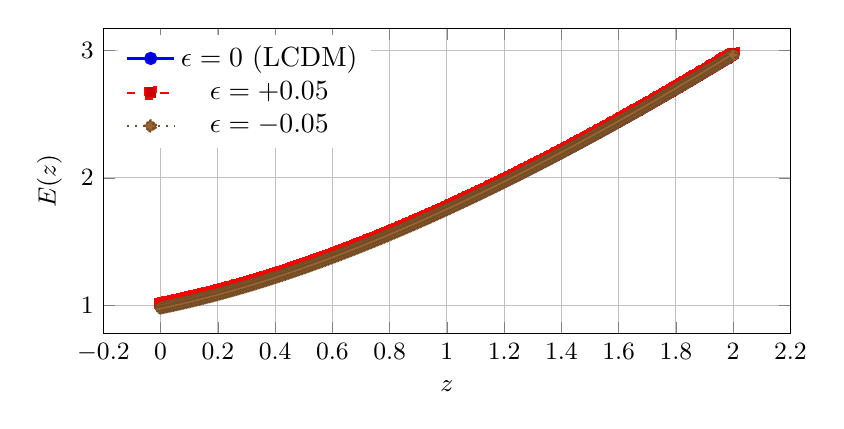
\begin{tikzpicture}
\begin{axis}[width=0.85\textwidth,height=0.45\textwidth,
xlabel={$z$}, ylabel={$E(z)$}, grid=both,
legend style={at={(0.02,0.98)},anchor=north west,fill=white,draw=none}, ticklabel style={font=\small}, label style={font=\small}]
\addplot+[domain=0:2.0,samples=400,thick] {sqrt(0.3*(1+x)^3 + 0.7*(1+0))};
\addlegendentry{$\epsilon=0$ (LCDM)}
\addplot+[domain=0:2.0,samples=400,thick,dashed] {sqrt(0.3*(1+x)^3 + 0.7*(1+0.05))};
\addlegendentry{$\epsilon=+0.05$}
\addplot+[domain=0:2.0,samples=400,thick,dotted] {sqrt(0.3*(1+x)^3 + 0.7*(1-0.05))};
\addlegendentry{$\epsilon=-0.05$}
\end{axis}
\end{tikzpicture}
\caption{Illustrative expansion histories with a small UBT dark-energy deformation $\epsilon=\kappa_\Lambda\psi$. For $\epsilon\to 0$ we recover $\Lambda$CDM.}
\label{fig:Hz}
\end{figure}

\section*{M.7 Observable Consequences (Qualitative)}
\begin{itemize}
\item Slight shifts in distance--redshift relations $D_L(z), D_A(z)$ and in the derived $H_0$ if $\epsilon\neq 0$ today.
\item Modified ISW effect and low-$\ell$ CMB for time-varying $\bar{\psi}(t)$.
\item Growth rate changes $f(z)\sigma_8$ suppressed by $c_{s,\rm UBT}^2\lesssim 1$; $\epsilon\to 0$ reproduces $\Lambda$CDM.
\end{itemize}

\section*{M.8 Relation to Psychon Sector and Local Tests}
The same $\psi$ that sources $\Lambda_{\rm eff}$ couples to local experiments (Appendix L/N). Constraints from cosmology (global $\bar{\psi}$) and laboratory (local $\psi$ modulations) are complementary; combined fits determine $(\kappa_\Lambda,M_\psi,\alpha_\psi)$ or bound them.

\section*{M.9 Summary}
UBT dark energy arises from a slow phase sector $\psi$ that perturbs the vacuum energy density and hence the effective cosmological constant. The framework recovers $\Lambda$CDM when the phase sector is inactive and predicts small, testable deviations otherwise. This ties cosmic acceleration to the same $\psi$ dynamics appearing in local UBT protocols.

\end{document}
